\documentclass{beamer}
\usepackage[utf8]{inputenc}
\usepackage{mathrsfs}  
\usepackage{xcolor}
\usepackage{setspace}
\usepackage{comment}

% config du thgeme metropolis
\usetheme[progressbar=frametitle,block=fill, titleformat=smallcaps,sectionpage=progressbar,]{metropolis}



\title{Distances}
\subtitle{}
\date{}
\author{paul}




%definition de la couleur du texte dans la balise \alert{}
\definecolor{vertIGN}{HTML}{96C31E} % vert IGN %vrai valeur #97BE0D
\setbeamercolor{alerted text}{fg=vertIGN}

\definecolor{grisIGN}{HTML}{22292F} % Gris IGN tiré vers le noir 
\setbeamercolor{background canvas}{bg=grisIGN}




% code pour placer le log ENSG dans le bandeau de titre 
\makeatletter
\setbeamertemplate{frametitle}{%
  \nointerlineskip%
  \begin{beamercolorbox}[%
      wd=\paperwidth,%
      sep=0pt,%
      leftskip=\metropolis@frametitle@padding,%
      rightskip=\metropolis@frametitle@padding,%
    ]{frametitle}%
  \metropolis@frametitlestrut@start%
  \insertframetitle%
  \nolinebreak%
  \metropolis@frametitlestrut@end%
  \hfill
  \raisebox{-0.6ex}{
\includegraphics[height=4ex,keepaspectratio]{img/logoENSG_small.jpg}}
  \end{beamercolorbox}%
}
\makeatother




% logo ENSG première page 
\titlegraphic{\vspace{4cm}\flushright
\includegraphics[width=2cm,height=2cm]{img/logoENSG_big.png}} 



\begin{document}
\metroset{background=dark} % change background theme according to manual
\maketitle  

\section{Going the distance} 

\begin{frame}{Various Distances}


$$d(A,B)$$

\begin{scriptsize}

is the quantification of 

\begin{itemize}
\item   «the quantity of 1D-space» between A and B , a \alert{"length"}, in something like meters
\item «similarity» between A and B, a \alert{metric} $\in \mathbb{R}$, sometimes $\in[0;1]$
\item  «quantity of separation» , as in the \alert{social distance} between two people in termes of classes  
\end{itemize}


$A,B$ may be sets, vectors in $\mathbb{R}^n$, doubles and strings and booleans

\end{scriptsize}

\end{frame}


\begin{frame}{My own distances taxonomy}



\begin{itemize}
\item  Physical Length : Geometry, Physics, Mecanics
\item  Error function :  Statistical model fitting 
\item  Fitness function : Genetic Algorithm
\item  Loss function : Machine Learning, Classification 
\item  Edit distance : Natural Language Processing, Info. Retrieval 
\item  Paths Lengths:  Graph theory, Optics, Acoustics
\item  Likelyhood : Probabilities 
\end{itemize}


\end{frame}



\begin{frame}{Disclaimer}


Due to \alert{curse of dimensionality}, there is no good distance in a high dimensional data
\end{frame}


\section{Distance as Physical Length}


\begin{frame}{Euclidean}

$$d(A,B)= \sqrt{\sum_{i}(A_i-B_i)^2} \in \mathbb{R}$$

\begin{scriptsize}

Requires \alert{cartesian coordinates} 



\begin{columns}[T,onlytextwidth]
\column{0.48\textwidth}
\begin{block}{Pros}
\begin{itemize}
  \item well known /widely used
  \item simple/intuitive
  \item perfect for 2D and 3D 
\end{itemize}
\end{block}
\column{0.4\textwidth}
\metroset{block=fill}
\begin{block}{Cons}
\begin{spacing}{0.9}
\begin{itemize}
  \item subject to scale/units 
  \item subject to curse of dimensionality 
  \item Earth is not flat
  \item high-dimensional data may include correlations beetween dimensions
\end{itemize}
\end{spacing}
\end{block}
\end{columns}


toy example : k-means on 2D points 
\end{scriptsize}

\end{frame}



\begin{frame}{Manhattan Distance}

$$d(A,B)= \sum_{i}|A_i-B_i| \in \mathbb{R}$$



\begin{scriptsize}
\begin{columns}[T,onlytextwidth]
\column{0.48\textwidth}
\begin{block}{Pros}
\begin{itemize}
  \item ok with high-dimensional data
  \item perfectly understandable if 1D ;-)
\end{itemize}
\end{block}
\column{0.4\textwidth}
\metroset{block=fill}
\begin{block}{Cons}
\begin{spacing}{0.9}
\begin{itemize}
  \item "not the shortest"
  \item hard to interpret
\end{itemize}
\end{spacing}
\end{block}
\end{columns}
\end{scriptsize}




\end{frame}



\begin{frame}{Chebyshev Distance}

$$d(A,B)= max_i |A_i-B_i| \in \mathbb{R}$$


\textit{"King distance"  on a chessboard}

\begin{scriptsize}
\begin{columns}[T,onlytextwidth]
\column{0.48\textwidth}
\begin{block}{Pros}
\begin{itemize}
  \item ? 
\end{itemize}
\end{block}
\column{0.4\textwidth}
\metroset{block=fill}
\begin{block}{Cons}
\begin{spacing}{0.9}
\begin{itemize}
  \item  other dimension than the one where max occurs don't count 
  \item hard to interpret
\end{itemize}
\end{spacing}
\end{block}
\end{columns}
\end{scriptsize}




\end{frame}




\begin{frame}{Minkowski Distance}

$$d(A,B)= \big(\sum_i|A_i-B_i|^p\big)^{\frac{1}{p}} \in \mathbb{R}$$


the \textit{"paramterizable norm"}

$p= 1$ : Manhatan

$p= 2$ : Euclidean 

$p = \infty$ : Chebyshev

\begin{scriptsize}
\begin{columns}[T,onlytextwidth]
\column{0.48\textwidth}
\begin{block}{Pros}
\begin{itemize}
  \item tunable with $p$ $\approx$ meta-parameters if used in model
\end{itemize}
\end{block}
\column{0.4\textwidth}
\metroset{block=fill}
\begin{block}{Cons}
\begin{spacing}{0.9}
\begin{itemize}
  \item shipped with others cons depending on values of p
  \item hard to interpret (what if $p=0.3$ ? )
\end{itemize}
\end{spacing}
\end{block}
\end{columns}
\end{scriptsize}




\end{frame}



\begin{frame}{Chebyshev Distance}

$$D_{M}(x)={\sqrt {(x-\mu )^{T}\Sigma ^{-1}(x-\mu )}}$$





\begin{scriptsize}
\begin{columns}[T,onlytextwidth]
\column{0.48\textwidth}
\begin{block}{Pros}
\begin{itemize}
  \item correlation taken into account
   \item  variance taken into account
\end{itemize}
\end{block}
\column{0.4\textwidth}
\metroset{block=fill}
\begin{block}{Cons}
\begin{spacing}{0.9}
\begin{itemize}
  \item distance between an element and \alert{a set of others}
  \item outliers sensitive (because variance and mean are)
\end{itemize}
\end{spacing}
\end{block}
\end{columns}
\end{scriptsize}




\end{frame}





\begin{frame}{Haversine Distance}


\begin{scriptsize}
$$d(A,B)=2r \arcsin  \sqrt{\sin ^{2} \left( {\frac{\varphi_{B}-\varphi_{A}}{2}}  \right) + cos(\varphi_A)cos(\varphi_B)\sin ^{2} \left( {\frac{\lambda_{B}-\lambda_{A}}{2}}  \right) }$$

$\varphi$ is latitude , $\lambda$ is longitude, $r$ is the sphere radius.


\begin{columns}[T,onlytextwidth]
\column{0.48\textwidth}
\begin{block}{Pros}
\begin{itemize}
  \item adapted for earth surface points
\end{itemize}
\end{block}
\column{0.4\textwidth}
\metroset{block=fill}
\begin{block}{Cons}
\begin{spacing}{0.9}
\begin{itemize}
  \item distortions if not on a regular sphere
  \item scary looking 
\end{itemize}
\end{spacing}
\end{block}
\end{columns}
\end{scriptsize}




\end{frame}



\section{Distance as Similarity}


\begin{frame}{Pearson'(s correlation)}


$$d(A,B)= \frac{cov(A,B)}{\sigma_A\sigma_B}=\frac{E\big[(A-E(A))(B-E(B))  \big]}{\sigma_A\sigma_B}$$ 



\begin{scriptsize}
\begin{columns}[T,onlytextwidth]
\column{0.48\textwidth}
\begin{block}{Pros}
\begin{itemize}
  \item very common
  \item normalised values $\in [-1;1]$
  \item used for high-dimensional data
\end{itemize}
\end{block}
\column{0.4\textwidth}
\metroset{block=fill}
\begin{block}{Cons}
\begin{spacing}{0.9}
\begin{itemize}
  \item captures "linearity" amount
  \end{itemize}
\end{spacing}
\end{block}
\end{columns}
\end{scriptsize}

\end{frame}


\section{Distance as Similarity}


\begin{frame}{Spearman's correlation}


$$d(A,B)= \frac{cov(rank_A, rank_B)}{\sigma_{rank_A}\sigma_{rank_B}}$$


Pearson on ranks 

\begin{scriptsize}
\begin{columns}[T,onlytextwidth]
\column{0.48\textwidth}
\begin{block}{Pros}
\begin{itemize}
  \item normalised values $\in [-1;1]$
  \item ok with monotonous trends
\end{itemize}
\end{block}
\column{0.4\textwidth}
\metroset{block=fill}
\begin{block}{Cons}
\begin{spacing}{0.9}
\begin{itemize}
  \item less known/used than Pearson 
  \end{itemize}
\end{spacing}
\end{block}
\end{columns}
\end{scriptsize}

\end{frame}




\begin{frame}{Cosine similarity}

$$d(A,B)= cos(\theta)= \frac{A.B}{||A||.||B||} \in[-1;1]$$

Requires \alert{scalar product}  and a \alert{norm}.


\begin{scriptsize}
\begin{columns}[T,onlytextwidth]
\column{0.48\textwidth}
\begin{block}{Pros}
\begin{itemize}
  \item still simple
  \item normalised values
  \item used for high-dimensional data
\end{itemize}
\end{block}
\column{0.4\textwidth}
\metroset{block=fill}
\begin{block}{Cons}
\begin{spacing}{0.9}
\begin{itemize}
  \item captures "orientation" only
  \item magnitudes  meaningless
  \item degraded by sparse data 
\end{itemize}
\end{spacing}
\end{block}
\end{columns}
\end{scriptsize}



\end{frame}


\begin{frame}{Hamming distance}

$$d(A,B)= Card\{i : A_i \neq B_i\}$$

\begin{center}
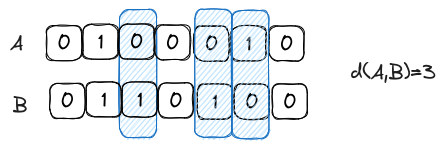
\includegraphics[width=0.5\textwidth,keepaspectratio]{img/hamming.png}
\end{center}

\begin{scriptsize}
The number of values that differ from A to B.


Requires \alert{same length} objects



\begin{columns}[T,onlytextwidth]
\column{0.48\textwidth}
\begin{block}{Pros}
\begin{itemize}
  \item intuitive (regarding objects size)
  \item simple 
\end{itemize}
\end{block}
\column{0.4\textwidth}
\metroset{block=fill}
\begin{block}{Cons}
\begin{spacing}{0.9}
\begin{itemize}
  \item same length constraint
  \item count differences occurences, not the \textit{gap}  
\end{itemize}
\end{spacing}
\end{block}
\end{columns}
\end{scriptsize}

use case : similarity using qualitative variables only

\end{frame}



\begin{frame}{Jaccard index}

$$d(A,B)= 1-\frac{A \cap B}{A \cup B} \in [0;1]$$

\begin{center}
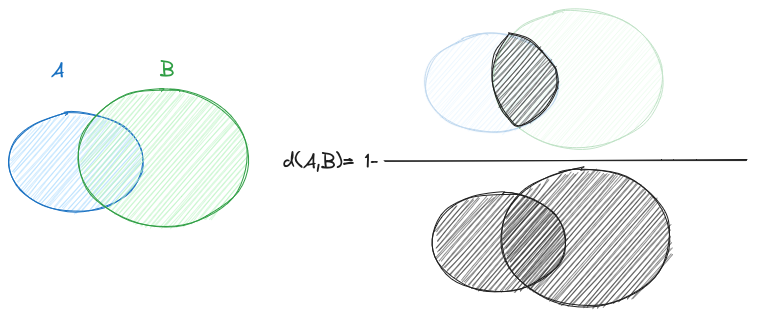
\includegraphics[width=0.5\textwidth,keepaspectratio]{img/jaccard.png}
\end{center}


\begin{scriptsize}
also called \alert{IOU}

Distance is 1- Jaccard index



\begin{columns}[T,onlytextwidth]
\column{0.48\textwidth}
\begin{block}{Pros}
\begin{itemize}
  \item intuitive : similarity of sets
  \item simple with cardinality
\end{itemize}
\end{block}
\column{0.4\textwidth}
\metroset{block=fill}
\begin{block}{Cons}
\begin{spacing}{0.9}
\begin{itemize}
  \item tend to be low for huge sets ($\cup$ is always big)
\end{itemize}
\end{spacing}
\end{block}
\end{columns}
\end{scriptsize}


use case : similarity between documents as common words count

\end{frame}








\begin{frame}{Kullback-Liebler divergence}

$$d(A,B)= \sum_{x \in X}A(x)log\frac{A(x)}{B(x)}$$

\begin{scriptsize}
$A$ and $B$ are probability  distributions on $X$ set

\begin{center}
%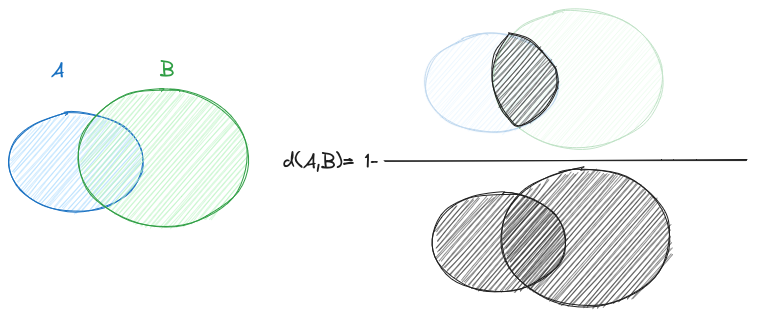
\includegraphics[width=0.5\textwidth,keepaspectratio]{img/jaccard.png}
\end{center}






\begin{columns}[T,onlytextwidth]
\column{0.48\textwidth}
\begin{block}{Pros}
\begin{itemize}
  \item well known
  \item  feat. entropy 
\end{itemize}
\end{block}
\column{0.4\textwidth}
\metroset{block=fill}
\begin{block}{Cons}
\begin{spacing}{0.9}
\begin{itemize}
  \item how to handle zeros in probabilities ? 
  \item $\implies$ additional smoothing required
  \item not a distance! (no symmetry + no triangle inequality)
  \item  strange if multimodalities
\end{itemize}
\end{spacing}
\end{block}
\end{columns}
\end{scriptsize}

\end{frame}



\begin{frame}{Overlapping index}


\begin{scriptsize}

$$d(A,B)= \int_{\mathbb{R}^n} min[f_A(x),f_B(x)]\ dx \in [0;1]$$


$f_A$ and $f_B$ are probability distribution functions

\begin{center}
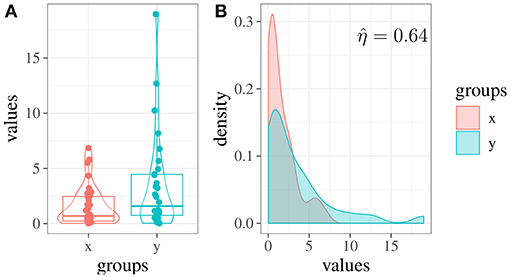
\includegraphics[width=0.3\textwidth,keepaspectratio]{img/overlappingindex.jpg}
\end{center}


dug by Kirana, thx! 



\begin{columns}[T,onlytextwidth]
\column{0.48\textwidth}
\begin{block}{Pros}
\begin{itemize}
  \item intuitive
  \item no distributions assumptions (unimodality, symmetry)
  \item works with different sizes samples
\end{itemize}
\end{block}
\column{0.4\textwidth}
\metroset{block=fill}
\begin{block}{Cons}
\begin{spacing}{0.9}
\begin{itemize}
  \item ?
\end{itemize}
\end{spacing}
\end{block}
\end{columns}
\end{scriptsize}

\begin{tiny}
\begin{singlespace}
Pastore, M., and Calcagnì, A. (2019).\href{https://www.frontiersin.org/articles/10.3389/fpsyg.2019.01089/full}{\color{cyan}{Measuring distribution similarities
between samples: a distribution-free overlapping index}}. Front. Psychol. 10:1089.
doi: 10.3389/fpsyg.2019.01089
\end{singlespace}
\end{tiny}

\end{frame}






\begin{frame}{}
%\centering

\end{frame}






\begin{frame}{Références}


TODO 

\begin{itemize}
\item \href{https://towardsdatascience.com/9-distance-measures-in-data-science-918109d069fa}{\color{cyan}{Initial blog post on Towards Data Science}}
\item \href{https://www.ijamtes.org/gallery/101.\%20nov\%20ijmte\%20-\%20as.pdf}{\color{cyan}{Goswami et al, A Comparative Analysis of Similarity Measures to find Coherent Documents}}

\end{itemize}


\end{frame}


\begin{comment}

\begin{frame}{Animation}
  \begin{itemize}[<+- | alert@+>]
    \item \alert<4>{This is\only<4>{ really} important}
    \item Now this
    \item And now this
  \end{itemize}
\end{frame}



\begin{frame}[standout]
Mono message sur une diapo
\end{frame}
\end{comment}

\end{document}
